%==============================================================
% PARTE 3: PASANDO A NIVEL INTERMEDIO
%==============================================================
\chapter{Parte 3: Pasando a Nivel Intermedio}

%--------------------------------------------------------------
\section{Crear un archivo launch}
%--------------------------------------------------------------

\subsection*{Pregunta 14}
\textit{¿Con qué nombre se han lanzado los nodos?}

Los nodos se han lanzado con los nombres \texttt{nodo\_envia} y \texttt{nodo\_recibe}, definidos en el campo \texttt{name} del fichero \texttt{mi\_launch.py}:

\begin{lstlisting}[style=python, caption={Fichero mi\_launch.py.}]
Node(package='primer_paquete', executable='server', name='nodo_envia'),
Node(package='primer_paquete', executable='client', name='nodo_recibe')
\end{lstlisting}

\begin{figure}[H]
  \centering
  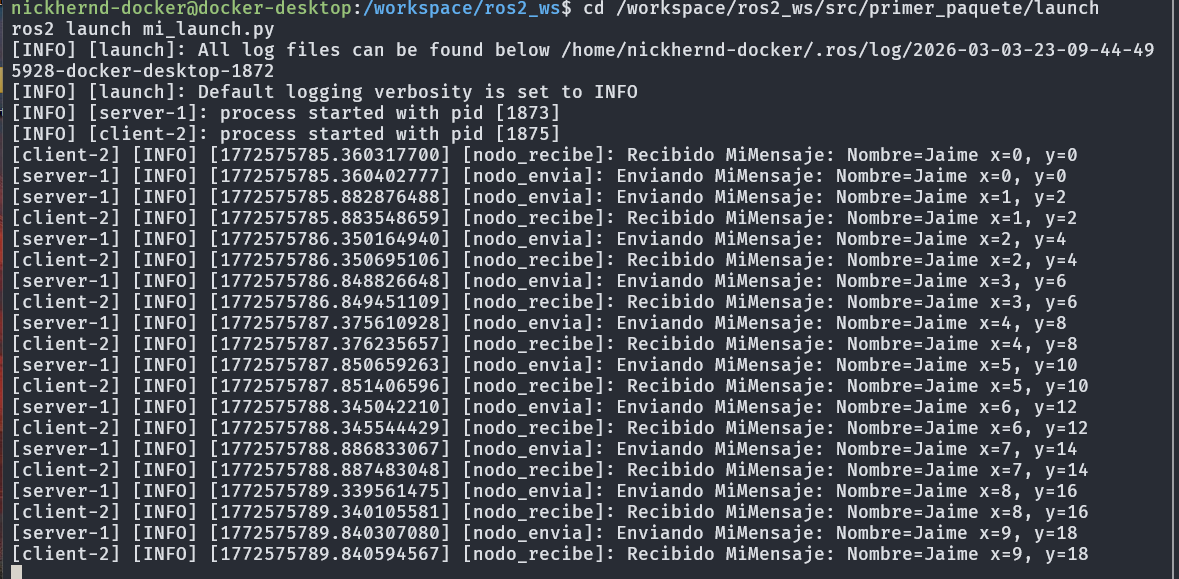
\includegraphics[width=0.85\textwidth]{parte3/imagenes/parte1.png}
  \caption{Nodos lanzados desde \texttt{mi\_launch.py} con sus nombres asignados.}
  \label{fig:p3_launch}
\end{figure}

%--------------------------------------------------------------
\section{Acciones}
%--------------------------------------------------------------

\subsection*{Pregunta 15}
\textit{¿Cómo podemos saber que se ha lanzado la acción correctamente? ¿Qué método permite saber que la acción ha finalizado exitosamente?}

La acción se ha lanzado correctamente cuando el servidor responde con \textit{goal accepted} y el cliente recibe el \texttt{goal\_id}. La acción finaliza exitosamente cuando el servidor ejecuta \texttt{goal\_handle.succeed()}, lo que dispara el callback \texttt{get\_result\_callback} en el cliente con el resultado final.

\begin{figure}[H]
  \centering
  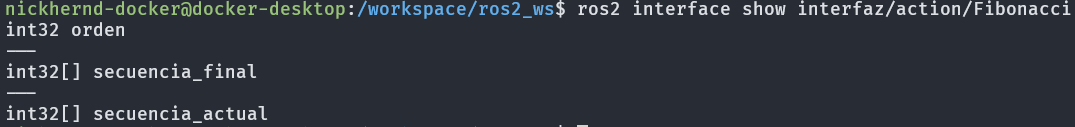
\includegraphics[width=0.85\textwidth]{parte3/imagenes/action_fibonacci.png}
  \caption{Servidor y cliente de la acción Fibonacci en ejecución.}
  \label{fig:p3_action}
\end{figure}

\subsection*{Pregunta 16}
\textit{Sin crear un nodo, ¿cómo lanzarías la acción Fibonacci? ¿Cómo observarías el resultado?}

Desde terminal, usando \texttt{ros2 action send\_goal} con el flag \texttt{--feedback} para ver el progreso:

\begin{lstlisting}[style=bash, caption={Lanzar la acción Fibonacci desde terminal.}]
ros2 action send_goal /fibonacci interfaz/action/Fibonacci \
    "{orden: 10}" --feedback
\end{lstlisting}

\begin{figure}[H]
  \centering
  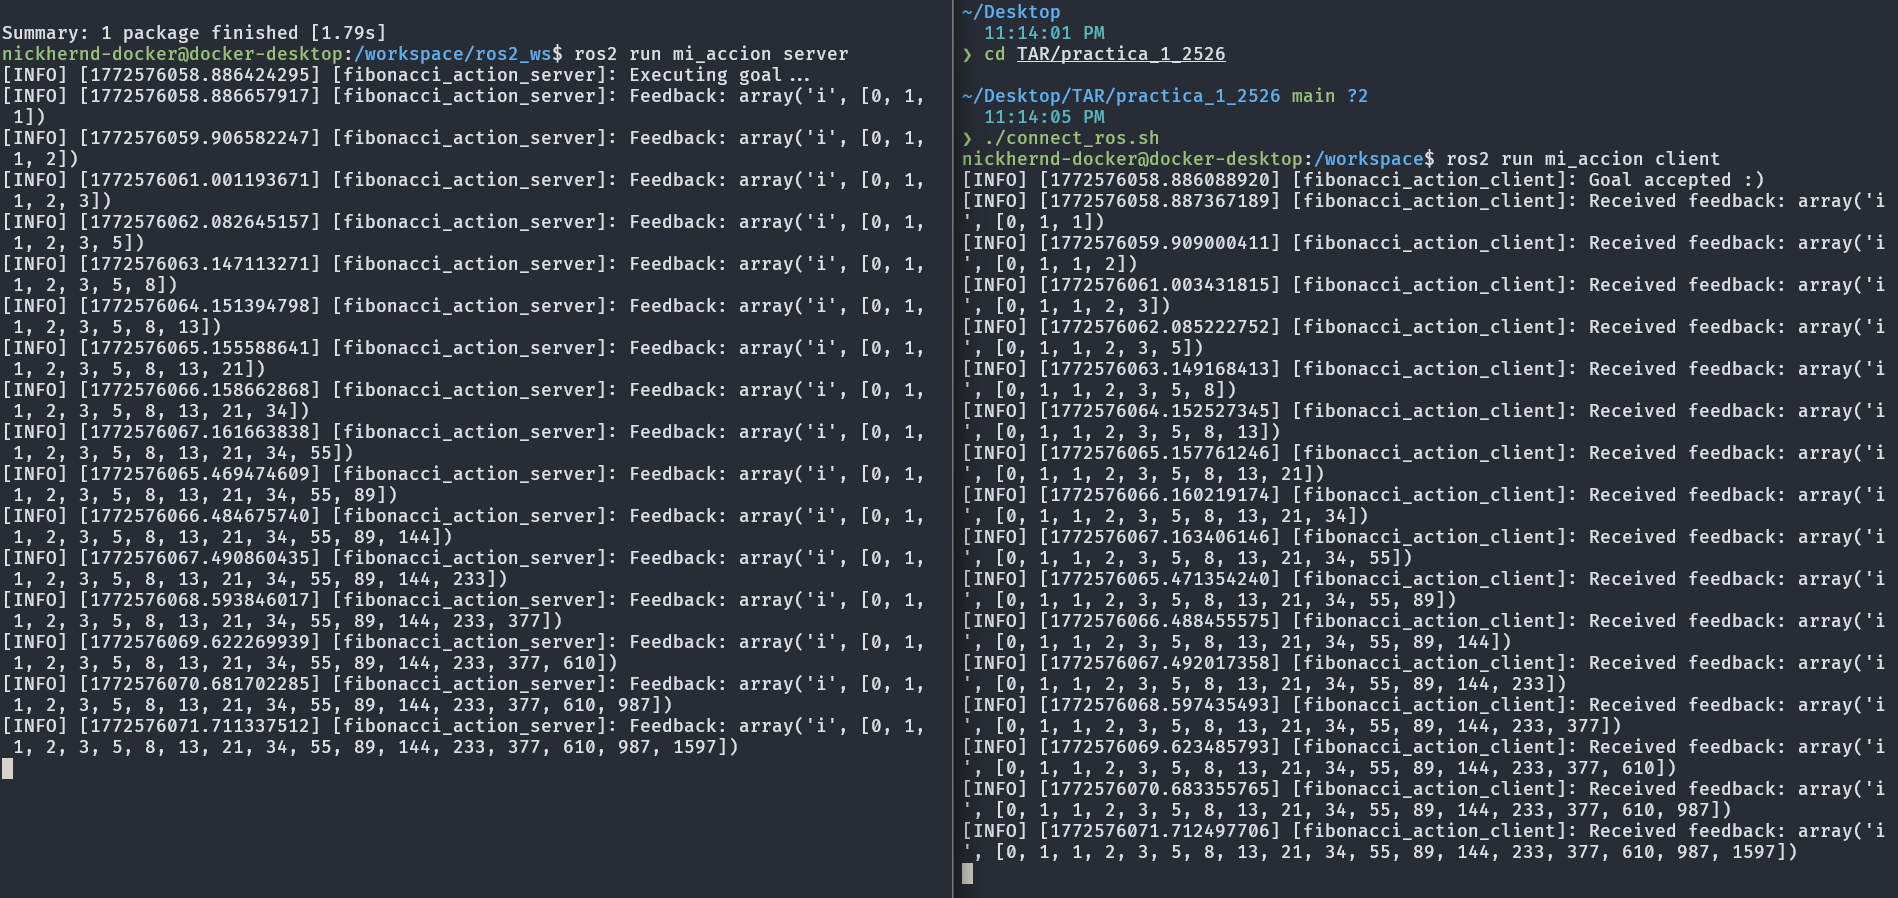
\includegraphics[width=0.85\textwidth]{parte3/imagenes/fib_accion_en_accion.png}
  \caption{Acción Fibonacci lanzada directamente desde terminal con feedback.}
  \label{fig:p3_action_terminal}
\end{figure}

\subsection*{Pregunta 17}
\textit{Si paramos el nodo a mitad de la ejecución, ¿se cancela la acción? ¿Se puede cancelar desde la terminal?}

Si se para el servidor (\texttt{Ctrl+C}), la acción no se cancela limpiamente: el cliente pierde la conexión y queda bloqueado sin recibir ni resultado ni cancelación. Sí se puede cancelar desde terminal mediante:
\begin{lstlisting}[style=bash]
ros2 action cancel <goal_uuid>
\end{lstlisting}
Siempre que el servidor tenga implementado un \texttt{cancel\_callback}.

%--------------------------------------------------------------
\section{Ejercicios}
%--------------------------------------------------------------

\subsection{Ejercicio 1: \texttt{launch\_ejercicio3.py}}

Fichero launch que lanza \texttt{nodopub\_ejercicio2} y \texttt{nodosub\_ejercicio2} con un argumento \texttt{numero} (por defecto 7) pasado como parámetro al publisher:

\begin{lstlisting}[style=python, caption={Argumento en launch\_ejercicio3.py.}]
numero_arg = DeclareLaunchArgument('numero', default_value='7')
Node(package='p2pkg', executable='nodopub_ejercicio2',
     parameters=[{'numero': LaunchConfiguration('numero')}])
\end{lstlisting}

\begin{figure}[H]
  \centering
  
\includegraphics[width=0.85\textwidth]{parte3/imagenes/ejercicio1.png}
  \caption{Ejecución de \texttt{launch\_ejercicio3.py} con argumento por defecto.}
  \label{fig:p3_ej1}
\end{figure}

\subsection{Ejercicio 2: \texttt{launch\_ejercicio4.py} con namespace y remapping}

Nota: listar nodos y topics

Los nodos se agrupan bajo el namespace \texttt{miGrupo} y se remapea el topic \texttt{/topic\_ejercicio2} a \texttt{/miGrupo/topic\_ejercicio2}:

\begin{lstlisting}[style=python, caption={Namespace y remapping en launch\_ejercicio4.py.}]
GroupAction([
    PushRosNamespace('miGrupo'),
    Node(..., remappings=[('/topic_ejercicio2',
                           '/miGrupo/topic_ejercicio2')]),
    ...
])
\end{lstlisting}

\begin{figure}[H]
  \centering
  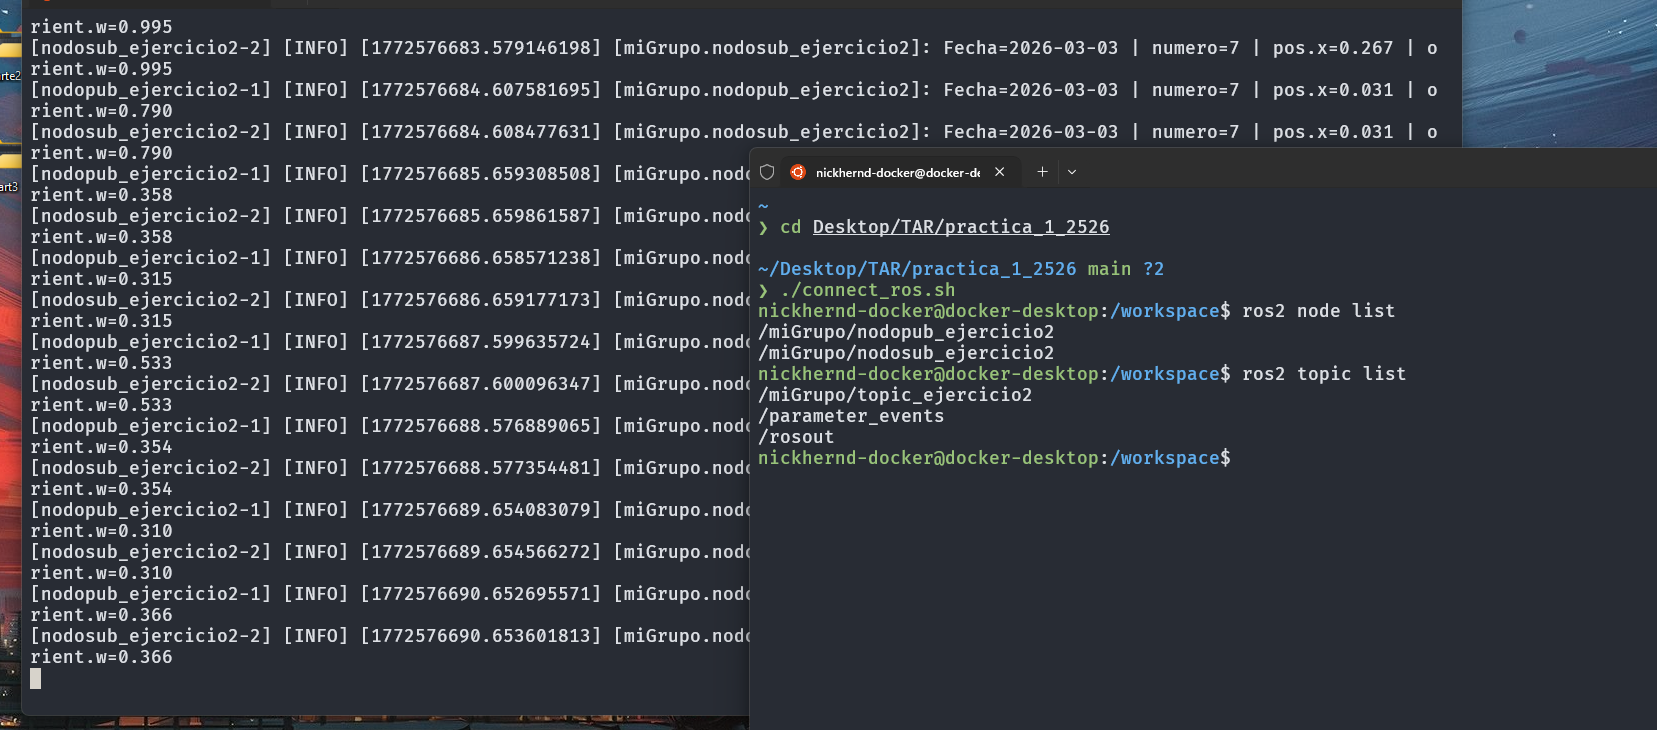
\includegraphics[width=0.85\textwidth]{parte3/imagenes/ejercicio2.png}
  \caption{\texttt{rqt\_graph} con nodos en el namespace \texttt{miGrupo}.}
  \label{fig:p3_ej2}
\end{figure}

\subsection{Ejercicio 3: Acción \texttt{EjFibonacci.action}}

Nueva acción con el mismo goal y result que \texttt{Fibonacci.action}, pero con feedback de tipo \texttt{float64}:

\begin{lstlisting}[caption={Definición de EjFibonacci.action.}]
int32 orden
---
int32[] secuencia_final
---
float64 feedback_value
\end{lstlisting}

\subsection{Ejercicio 4: Servidor \texttt{ejercicios\_fibServer.py}}

El servidor calcula la secuencia de Fibonacci y en cada iteración envía como feedback la raíz cuadrada de la media de la secuencia calculada hasta ese momento:

\begin{lstlisting}[style=python, caption={Cálculo del feedback en el servidor.}]
media = sum(secuencia) / len(secuencia)
feedback_msg.feedback_value = math.sqrt(media)
goal_handle.publish_feedback(feedback_msg)
\end{lstlisting}

\begin{figure}[H]
  \centering
  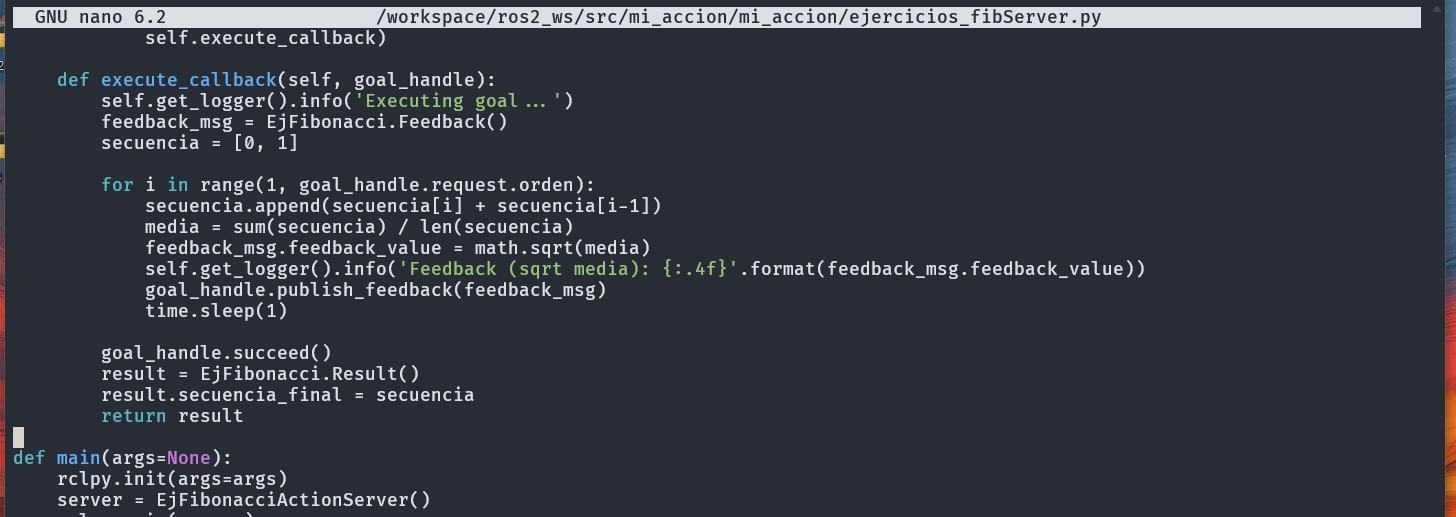
\includegraphics[width=0.85\textwidth]{parte3/imagenes/ejercicio4.png}
  \caption{Servidor \texttt{ejfibonacci\_action\_server} publicando feedback.}
  \label{fig:p3_ej4}
\end{figure}

\subsection{Ejercicio 5: Cliente \texttt{ejercicios\_fibClient.py}}

El cliente acepta el orden como argumento por línea de comandos y, mientras la acción está en curso, publica periódicamente el string \texttt{'en proceso'} en el topic \texttt{/estado\_accion}:

\begin{lstlisting}[style=python, caption={Publicación del estado mientras la acción está en curso.}]
def publish_estado(self):
    if self._in_progress:
        msg = String()
        msg.data = 'en proceso'
        self._publisher.publish(msg)
\end{lstlisting}

\begin{figure}[H]
  \centering
  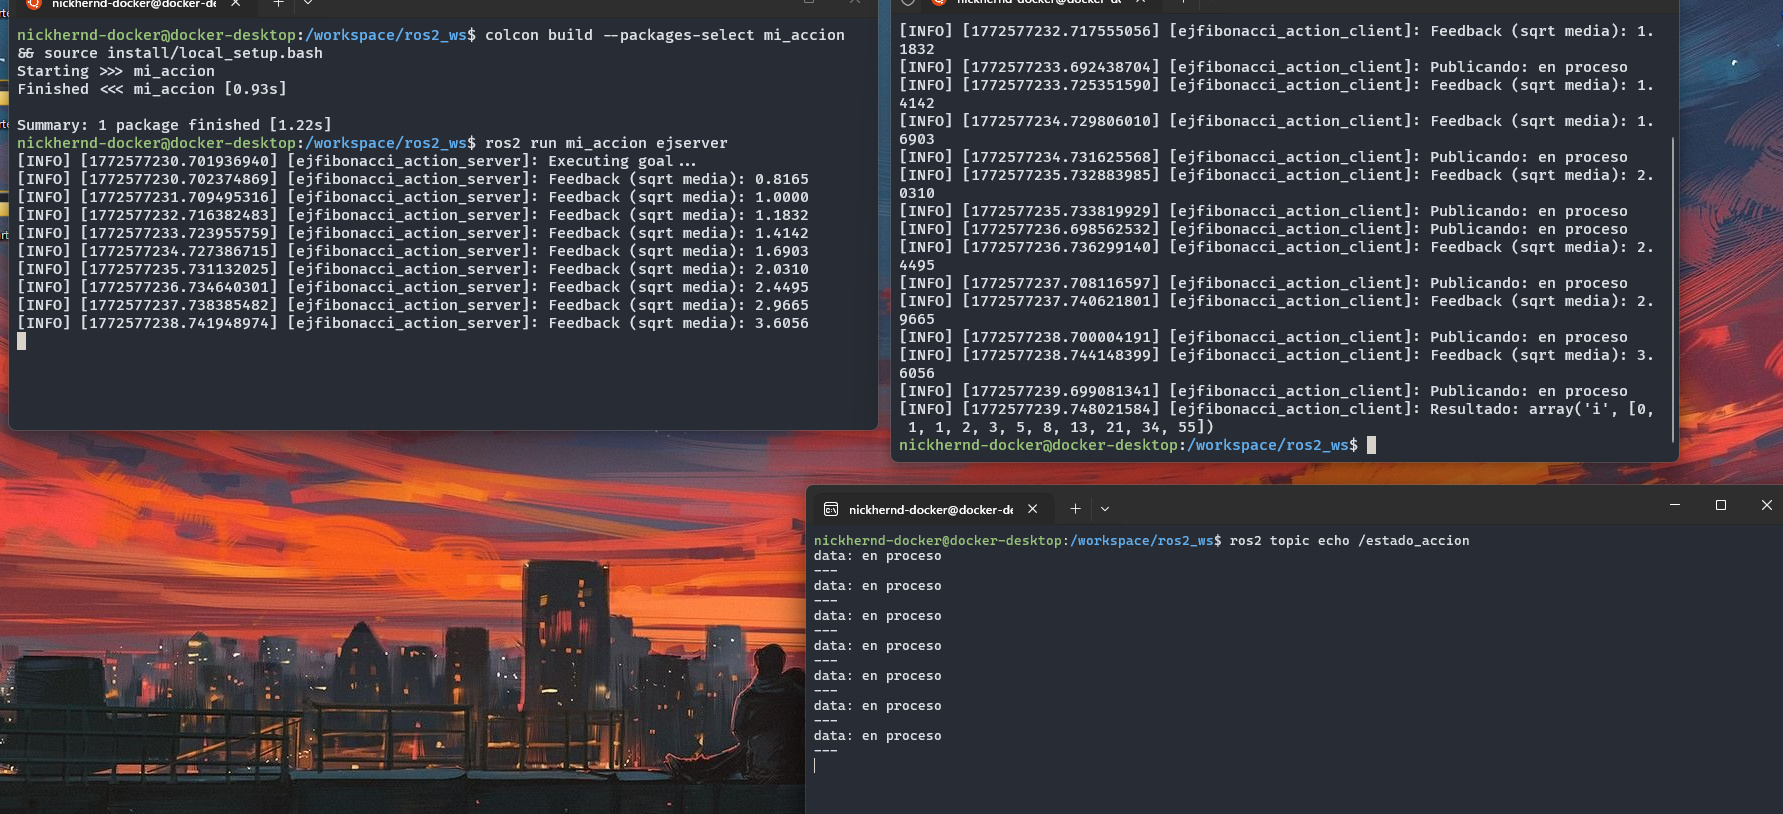
\includegraphics[width=0.85\textwidth]{parte3/imagenes/ejercicio5.png}
  \caption{Cliente recibiendo feedback y publicando estado en \texttt{/estado\_accion}.}
  \label{fig:p3_ej5}
\end{figure}

\subsection{Ejercicio 6: Servicio \texttt{service\_temp} (conversión de temperatura)}

Servicio que convierte entre Celsius y Fahrenheit según el campo \texttt{conversion\_type}:

\textbf{Interfaz} (\texttt{TempConversion.srv}):
\begin{lstlisting}[caption={Interfaz del servicio de temperatura.}]
float64 input_temp
string conversion_type   # "Cel_to_Far" o "Far_to_Cel"
---
float64 converted_temp
\end{lstlisting}

Las conversiones implementadas son:
\begin{itemize}
  \item \texttt{Cel\_to\_Far}: $T_F = T_C \times \frac{9}{5} + 32$
  \item \texttt{Far\_to\_Cel}: $T_C = (T_F - 32) \times \frac{5}{9}$
\end{itemize}

\begin{figure}[H]
  \centering
  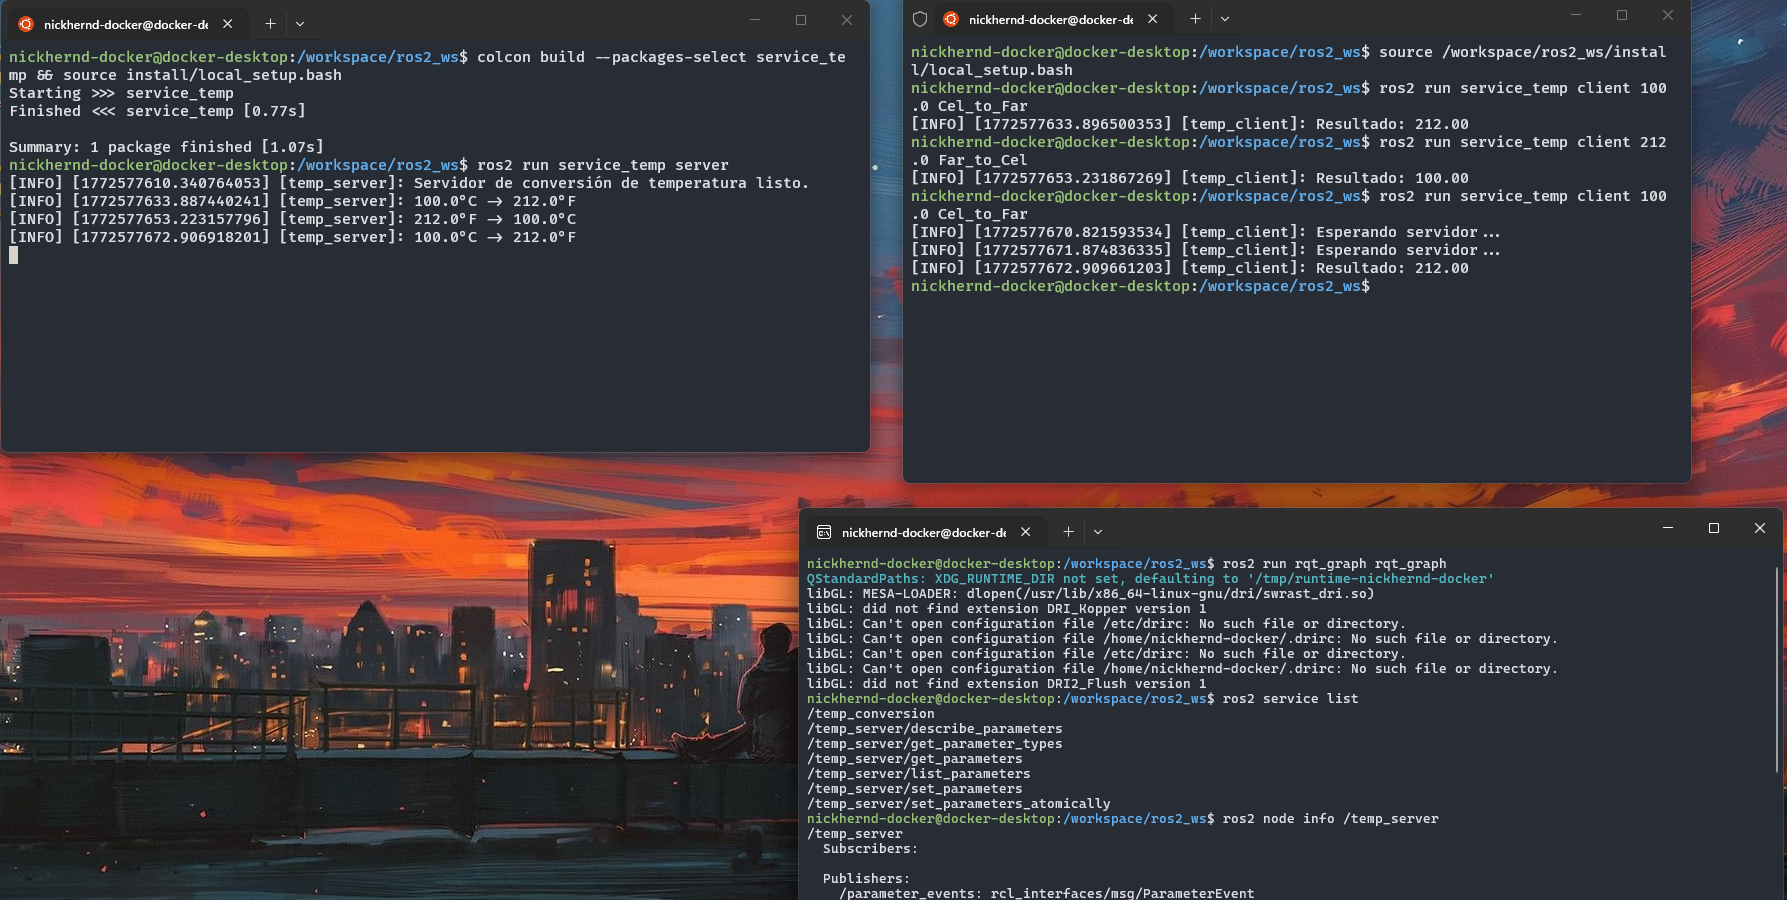
\includegraphics[width=0.85\textwidth]{parte3/imagenes/ejercicio6_finish.png}
  \caption{Ejecución del servicio de conversión de temperatura.}
  \label{fig:p3_ej6}
\end{figure}

\subsection{Ejercicio 7: Acción \texttt{battery\_act} (simulación de batería)}

Sistema que simula la descarga de la batería de un robot desde 100\% hasta un porcentaje objetivo.

\textbf{Interfaz} (\texttt{BatteryAction.action}):
\begin{lstlisting}[caption={Interfaz de la acción battery\_act.}]
int32 target_percentage
---
string warning
---
int32 current_percentage
\end{lstlisting}

El servidor (\texttt{battery\_charger}) decrementa la batería en 5\% cada segundo, publicando el nivel actual como feedback. Al alcanzar el objetivo, devuelve el mensaje de aviso \textit{``¡Batería baja, por favor cargue el robot!''}. Admite cancelación en cualquier momento gracias al \texttt{cancel\_callback}.

\begin{figure}[H]
  \centering
  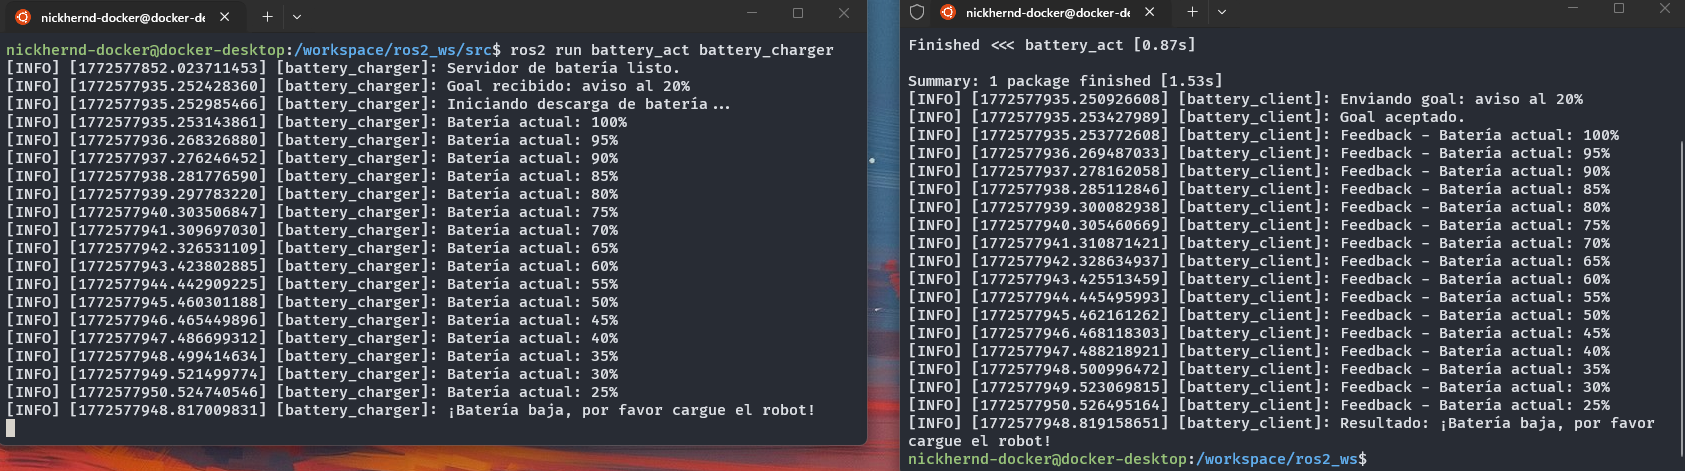
\includegraphics[width=0.85\textwidth]{parte3/imagenes/ejercicio7.png}
  \caption{Servidor \texttt{battery\_charger} y cliente \texttt{battery\_client} en ejecución.}
  \label{fig:p3_ej7}
\end{figure}
